\chapter{METODOLOGÍA DE LA INVESTIGACIÓN}
\section{Diseño de la investigación}
En el presente capítulo se define el diseño, tipo y enfoque de la investigación. Asimismo, se explica la población y muestra, es decir la base de dato que va a ser usada. Finalmente, se explican las técnicas usadas para la recolección de datos, el preprocesamiento de los mismos y el modelo Deep Learning para la creación del modelo de clasificación.
\subsection{Diseño experimental}
El diseño de la presente investigación es de tipo cuasi-experimental, ya que no se puede realizar una asignación aleatoria de los sujetos en el entorno de tienda retail. Se implementará un sistema de recomendación en el cual se utilizará el modelo de visión por computadora YOLO (You Only Look Once) para la detección y seguimiento de clientes en la tienda. A partir de los datos recopilados, se generará un mapa de calor que permita identificar las áreas de mayor y menor flujo de clientes. Este mapa de calor servirá como insumo para el sistema de recomendación de redistribución de productos en los anaqueles, buscando optimizar el flujo de clientes y lograr una distribución más uniforme en la tienda. El sistema ajustará la disposición de los productos para balancear el tráfico en el espacio de tienda y mejorar la experiencia de compra.

\subsection{Tipo explicativo}
El nivel del trabajo de investigación es explicativo, debido a que el diseño de un sistema de visión por computadora para el sistema de recomendación en el sector retail busca comprender la relación causa efecto entre la implementación del sistema y los resultados obtenidos, es decir como las recomendaciones generadas por el sistema basado en visión por computadora afectan la disposición de los productos, las ventas y la experiencia del cliente. Este enfoque es coherente con lo descrito por Sampieri et al. (2014), quienes señalan que el nivel explicativo busca identificar las causas de un fenómeno y sus efectos, aportando comprensión sobre las condiciones que determinan su ocurrencia.

\subsection{Enfoque cuantitativo}
El enfoque de la investigación es cuantitativo, debido a que se utilizan instrumentos para la identificación y medición del objeto de estudio el cual es el sistema de recomendación para el sector retail a través del recorrido de los clientes, se utilizaran la técnica de visión por computadora (YOLO) cuyos resultado numéricos servirán como el tiempo de permanencia de los clientes en la tienda para el mapa de calor por zonas, la precisión del modelo como la precisión, recall, F1-score y tiempo del procesamiento, serán analizados. Según Sampieri, Fernández y Baptista (2014), la investigación cuantitativa permite medir fenómenos y realizar análisis estadísticos para generalizar resultados, lo que asegura la objetividad en la interpretación de los datos obtenidos.

\section{Población y muestra}

\begin{table}[H]
\centering

\begin{tabular}{|>{\raggedright}p{3.5cm}|p{10cm}|}
\hline
\textbf{Población} & La población de esta investigación está compuesta por tiendas retail pequeñas y medianas que cuentan con cámaras de vigilancia en diversas regiones del Perú. Estas tiendas utilizan sistemas de grabación para aplicar técnicas de visión por computadora como YOLO, optimizando la distribución de productos y mejorando la experiencia del cliente. \\ \hline
\textbf{Muestra}   & 50 videos de videovigilancia corresponde al minimarket “La Económica”, ubicado en Puquio, provincia de Lucanas, Ayacucho, Perú. Este minimarket cuenta videos que captura videos del comportamiento de los clientes en distintas zonas del establecimiento. Los datos obtenidos se utilizarán para aplicar el método YOLO y generar recomendaciones sobre la redistribución de productos en bloques de zonas. El muestreo es no probabilístico por conveniencia, dado el acceso a datos relevantes. \\ \hline
\textbf{Unidad de Análisis}  & Cada video de vigilancia capturado será una unidad de análisis, de la cual se extraerán métricas clave como la distribución del tiempo de permanencia de los clientes en diferentes zonas de la tienda. \\ \hline
\textbf{Variables y Tipos de Variables}  & Las variables analizadas serán cuantitativas y continuas, centradas en datos numéricos como el tiempo de permanencia, la precisión del modelo y otras métricas de rendimiento. \\ \hline
\end{tabular}
\caption{Tabla de Población y la Muestra}
\label{tab:poblacion_muestra}
\end{table}


\section{Operacionalización de Variables}

\begin{table}[H]
\centering
\begin{tabular}{|>{\raggedright}p{3.5cm}|p{5cm}|p{5.5cm}|}
\hline
\textbf{VARIABLE Y DEFINICIÓN} & \textbf{INDICADOR} & \textbf{FÓRMULA} \\ \hline

\textbf{Sistema de Recomendacion de Productos.}
%Generación de sugerencias para mejorar la distribución de productos en función del análisis de los videos.
& Efectividad de las recomendaciones & $\frac{\text{Incremento de ventas post-recomendación}}{\text{Ventas previas}}$  \\ \cline{2-3}&Aumento en tiempo de permanencia en zonas recomendadas & 
$\frac{\text{Tiempo en zonas recomendadas}}{\text{Tiempo total en la tienda}}$ \\ \hline

\textbf{Visión por Computadora} & Resolución del video. & Cantidad de pixeles encontrados en el video \\ \cline{2-3} & Procesamiento del video & Nivel de nitidez, contraste o ruido encontrado en la imagen\\ \hline
 
\textbf{Modelo de Clasificación} & Accuracy & $\frac{TP + TN}{TP + FP + FN + TN}$ \\ \cline{2-3} 
& Precisión & $\frac{TP}{TP + FP}$ \\ \cline{2-3} 
& Recall & $\frac{TP}{TP + FN}$ \\ \cline{2-3} 
& F1 & $2 \cdot \frac{\text{Precisión} \cdot \text{Recall}}{\text{Precisión} + \text{Recall}}$ \\ \hline
% & ROC AUC & $P(\text{score}(x^+) > \text{score}(x^-))$ \\ \hline
\end{tabular}
\caption{Definición de variables}
\label{tab:definicion_variables}
\end{table}

Donde:
\begin{itemize}
    \item TP: Verdaderos Positivos.
    \item FP: Falsos Positivos.
    \item TN: Verdaderos Negativos.
    \item FN: Falsos Negativos.
\end{itemize}


\section{Técnicas de recolección de datos}

En esta sección se describen las técnicas empleadas para la recolección de datos visuales y demográficos, los cuales son esenciales para desarrollar el sistema de visión por computadora propuesto.

\subsection{Configuración Inicial}

Para la recolección de datos se instalaron cámaras de visión estándar en ``La Económica''. Se definieron tres áreas de interés: zona de entrada, pasillo central y área de cajas. Estas áreas se eligieron en base al flujo promedio de clientes observado.

\subsection{Procedimientos de Recolección}

\begin{table}[H]
\centering
\caption{Actividades para la recolección de datos}
\label{table:recoleccion}
\begin{tabular}{|p{5cm}|p{10cm}|}
\hline
\textbf{Actividad} & \textbf{Descripción} \\ \hline
\textbf{Grabación inicial} & Las cámaras capturaron datos en intervalos de 15 fps durante las horas pico (10:00 a 13:00 y 17:00 a 20:00) por un periodo de 14 días. \\ \hline
\textbf{Segmentación de video} & Se segmentaron los videos en intervalos de 10 segundos para analizar patrones individuales de clientes. \\ \hline
\textbf{Etiquetado manual} & Un equipo de 3 personas etiquetó manualmente las zonas transitadas utilizando software especializado como LabelImg. \\ \hline
\textbf{Validación de datos} & Los datos etiquetados fueron validados por un especialista en análisis de comportamiento en tiendas retail. \\ \hline
\end{tabular}
\end{table}

\subsection{Instrumentos Utilizados}

\begin{itemize}
    \item \textbf{Cámaras de visión estándar:} Configuradas con resolución 1080p y un ángulo de visión de 90 grados.
    \item \textbf{Software de etiquetado:} LabelImg para crear conjuntos de datos anotados que incluyan información como zonas de alto y bajo tránsito.
    
\end{itemize}

\textbf{Entregables:} Conjunto de datos etiquetados con información de flujo de clientes y zonas transitadas.

\subsection{Precisión en la Recolección de Datos}

Para garantizar la calidad de los datos recolectados, se calcularon métricas de confiabilidad:

\begin{equation}
\text{Precisión en etiquetado} = \frac{\text{Etiquetas correctas validadas}}{\text{Total de etiquetas generadas}} \times 100
\end{equation}

\begin{equation}
\text{Cobertura de cámaras} = \frac{\text{Área cubierta por cámaras}}{\text{Área total de la tienda}} \times 100
\end{equation}

\textbf{Resultados esperados:}
- Cobertura del 85\% de las áreas clave de la tienda.
- Precisión del 90\% en el etiquetado manual de los datos recolectados.

% Nisi porta lorem mollis aliquam ut porttitor leo. Aenean pharetra magna ac placerat vestibulum. Est placerat in egestas erat imperdiet sed euismod. Velit euismod in pellentesque massa placerat. Enim praesent elementum facilisis leo vel fringilla. Ante in nibh mauris cursus mattis molestie a iaculis. Erat pellentesque adipiscing commodo elit at imperdiet dui accumsan sit. Porttitor lacus luctus accumsan tortor posuere ac ut. Tortor at auctor urna nunc id. A iaculis at erat pellentesque adipiscing commodo elit.

% \LaTeX{} is great at typesetting mathematics. Let $X_1, X_2, \ldots, X_n$ be a sequence of independent and identically distributed random variables with
% \begin{equation}
% 	S_n = \frac{X_1 + X_2 + \cdots + X_n}{n}
% 	= \frac{1}{n}\sum_{i}^{n} X_i
% 	\label{eq1}
% \end{equation}

% La Ecuación \ref{eq1} denote their mean. Then as $n$ approaches infinity, the random variables $$\sqrt{n}(S_n - \mu)$$ converge in distribution to a normal $\mathcal{N}(0, \sigma^2)$.

\section{Técnicas para el Procesamiento y Análisis de la Información}

\subsection{Metodología de Implementación de la Solución}

Según Szeliski (2010), las etapas fundamentales en un sistema de visión por computadora incluyen la adquisición, preprocesamiento, extracción de características, y modelado. En este proyecto, estas etapas han sido adaptadas para resolver el problema de optimización en la distribución de productos en tiendas retail, como se detalla a continuación.
\begin{figure}[H]
    \centering
    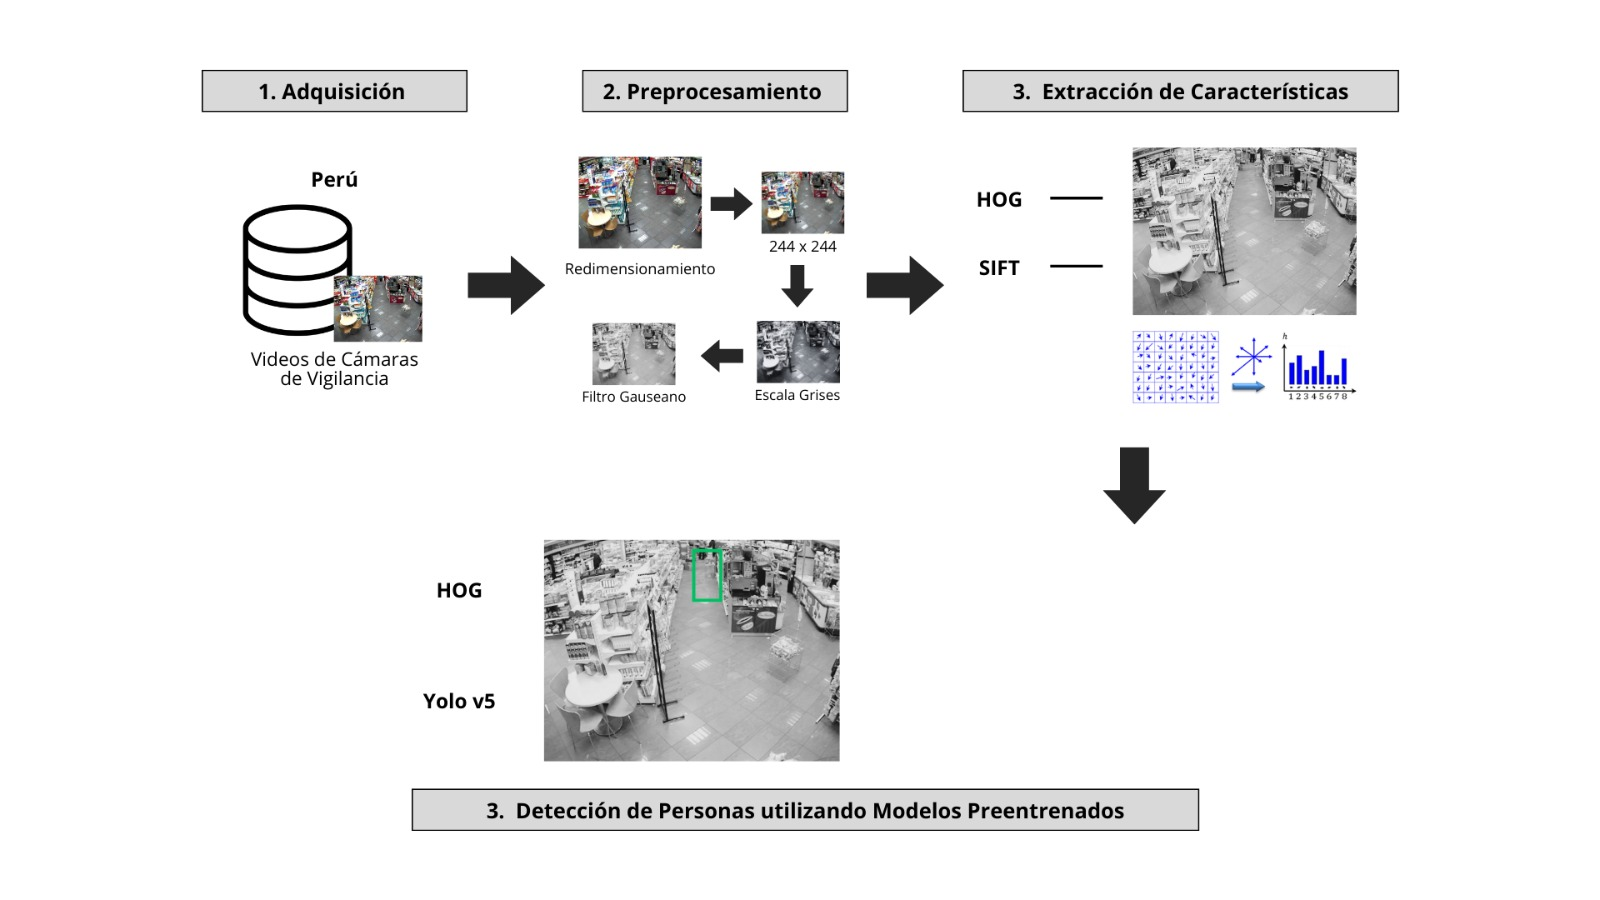
\includegraphics[width=0.8\textwidth]{3/figures/metodologia1.jpg} % Ajusta el tamaño y ruta
    \caption{Metodología}
    \label{fig:etiqueta_imagen} % Para referenciar la imagen en el texto
\end{figure}
\subsubsection{Adquisición}

La adquisición de datos fue realizada mediante la instalación de cámaras de visión estándar en el negocio retail ``La Económica'', recopilando imágenes de las áreas de interés clave. Estas cámaras se configuraron para registrar imágenes de 1080p con una frecuencia de 15 fps.

\begin{table}[H]
\centering
\caption{Actividades etapa de adquisición}
\label{table:adquisicion}
\begin{tabular}{|p{5cm}|p{8cm}|}
\hline
\textbf{Actividades} & \textbf{Descripción} \\ \hline
Identificación de áreas clave & Selección de zonas con alta densidad de tránsito de clientes. \\ \hline
Configuración de cámaras & Instalación y calibración de cámaras para capturar datos relevantes. \\ \hline
Grabación inicial & Grabación continua durante horarios pico por un periodo de 14 días. \\ \hline
\end{tabular}
\end{table}

\textbf{Entregables:} Datos en formato de video y frames estáticos clasificados por ubicación y rango horario.

\subsubsection{Preprocesamiento}

El preprocesamiento consistió en la normalización y mejora de las imágenes adquiridas. Se utilizaron técnicas como:

\begin{itemize}
    \item \textbf{Redimensionamiento:} Ajuste de las imágenes a $224 \times 224$ píxeles para compatibilidad con modelos.
    \item \textbf{Conversión a escala de grises:} Reducción de la dimensionalidad de los datos.
    \item \textbf{Eliminación de ruido:} Aplicación de filtros de mediana y gaussiano.
    \item \textbf{Data augmentation:} Incremento de la diversidad mediante rotaciones, traslaciones y ajustes de brillo.
\end{itemize}

\begin{equation}
I'(x, y) = \frac{I(x, y) - \text{min}(I)}{\text{max}(I) - \text{min}(I)} \times 255
\label{eq:normalization}
\end{equation}

\subsubsection{Extracción de Características}

Se implementaron técnicas avanzadas de extracción de características para identificar patrones relevantes en las imágenes:

\begin{table}[H]
\centering
\caption{Técnicas de extracción de características utilizadas}
\label{table:features}
\begin{tabular}{|l|p{10cm}|}
\hline
\textbf{Técnica} & \textbf{Descripción} \\ \hline
HOG (Histogram of Oriented Gradients) & Permite detectar bordes y gradientes locales. \\ \hline
SIFT (Scale-Invariant Feature Transform) & Detecta puntos de interés robustos a escala y rotación. \\ \hline
\end{tabular}
\end{table}

\subsubsection{Detección de Personas utilizando Modelos Preentrenados}

En esta etapa del proceso, la detección de personas se lleva a cabo mediante el uso de modelos ya entrenados, aprovechando arquitecturas probadas y reconocidas en el estado del arte, específicamente \textbf{HOG} (Histogram of Oriented Gradients), \textbf{SIFT} (Scale-Invariant Feature Transform) y \textbf{YOLOv5} (You Only Look Once, versión 5). Estas técnicas permiten identificar y localizar a las personas dentro de las imágenes sin necesidad de desarrollar un modelo propio mediante entrenamiento, validación o prueba. 

\paragraph{Detección con HOG.} El modelo de \textit{Histogram of Oriented Gradients (HOG)}, preentrenado para la detección de personas, se utiliza para extraer características visuales basadas en gradientes locales. El HOG genera un descriptor robusto que facilita la identificación de formas humanas, incluso en condiciones de iluminación variables. Este modelo preentrenado permite una detección confiable al aplicar directamente su clasificador lineal sobre las características calculadas.

\paragraph{Detección con SIFT.} La técnica \textit{Scale-Invariant Feature Transform (SIFT)} es empleada para identificar puntos de interés clave en las imágenes. Aunque SIFT no está específicamente diseñado para la detección de personas, su integración como un método de extracción de características complementa los resultados de HOG al detectar patrones invariantes a escala y rotación que están presentes en las siluetas humanas.

\paragraph{Detección con YOLOv5.} \textit{You Only Look Once, versión 5 (YOLOv5)} es un modelo preentrenado para la detección en tiempo real de personas. Este modelo, ampliamente optimizado y eficaz, permite localizar objetos específicos (en este caso, personas) mediante bounding boxes en las imágenes. Gracias a su enfoque basado en regresión, YOLOv5 identifica simultáneamente la clase del objeto y sus coordenadas espaciales. Al ser una solución preentrenada, su implementación se limita a la inferencia, sin necesidad de ajustes adicionales.

\paragraph{Implementación General.} La integración de estos modelos se realiza con herramientas preexistentes y bien documentadas, como bibliotecas de Python (\textit{OpenCV, TensorFlow, PyTorch}). A través de ellas, las imágenes del dataset se procesan directamente para obtener las detecciones de personas, siguiendo el flujo definido en la metodología. Este enfoque elimina la necesidad de separar el dataset en subconjuntos de entrenamiento, validación y prueba, dado que los modelos preentrenados ya contienen la información requerida para la detección eficiente.

\begin{figure}[H]
    \centering
    \includegraphics[width=0.8\textwidth]{ruta_a_diagrama}
    \caption{Flujo de detección de personas utilizando modelos preentrenados (HOG, SIFT y YOLOv5).}
    \label{fig:deteccion_personas}
\end{figure}

Este esquema metodológico asegura una detección precisa y eficiente de personas, empleando herramientas consolidadas y reduciendo la carga computacional asociada al entrenamiento de modelos desde cero.


\section{Medición de Resultados}

Para evaluar el desempeño del sistema, se utilizaron las métricas estándar de clasificación:

\begin{equation}
\text{Accuracy} = \frac{TP + TN}{TP + TN + FP + FN}
\end{equation}

\begin{equation}
\text{Precision} = \frac{TP}{TP + FP}, \quad \text{Recall} = \frac{TP}{TP + FN}
\end{equation}

Donde:
\begin{itemize}
    \item TP: Verdaderos Positivos.
    \item FP: Falsos Positivos.
    \item TN: Verdaderos Negativos.
    \item FN: Falsos Negativos.
\end{itemize}

\section{Cronograma de Actividades}

El cronograma se desarrolló considerando las fases principales del proyecto, distribuidas a lo largo de 9 meses.

\begin{table}[H]
\centering
\caption{Cronograma de actividades}
\label{table:cronograma}
\begin{tabular}{|p{4cm}|p{8cm}|}
\hline
\textbf{Fase} & \textbf{Meses y Actividades} \\ \hline
Adquisición de datos & Enero - Febrero: Configuración de cámaras y recolección inicial de imágenes. \\ \hline
Preprocesamiento & Marzo - Abril: Limpieza y normalización de datos. \\ \hline
Entrenamiento y Validación & Mayo - Julio: Entrenamiento de modelos y validación de resultados. \\ \hline
Evaluación y Documentación & Agosto - Septiembre: Evaluación del sistema, generación de conclusiones y recomendaciones. \\ \hline
\end{tabular}
\end{table}

\section{Presupuesto}

\begin{table}[H]
\centering
\caption{Presupuesto estimado del proyecto}
\label{table:presupuesto}
\begin{tabular}{|l|p{7cm}|r|}
\hline
\textbf{Recurso} & \textbf{Descripción} & \textbf{Costo (S/.)} \\ \hline
Cámaras & Cámaras de alta resolución para captura de datos & 1200 \\ \hline
Software & Licencias de herramientas como TensorFlow y PyTorch & 0 \\ \hline
Consultoría & Expertos en visión por computadora & 800 \\ \hline
\end{tabular}
\end{table}
% Nisi porta lorem mollis aliquam ut porttitor leo. Aenean pharetra magna ac placerat vestibulum. Est placerat in egestas erat imperdiet sed euismod. Velit euismod in pellentesque massa placerat. Enim praesent elementum facilisis leo vel fringilla. Ante in nibh mauris cursus mattis molestie a iaculis. Erat pellentesque adipiscing commodo elit at imperdiet dui accumsan sit. Porttitor lacus luctus accumsan tortor posuere ac ut. Tortor at auctor urna nunc id. A iaculis at erat pellentesque adipiscing commodo elit.

% You can make lists with automatic numbering \dots

% \begin{enumerate}
% 	\item Like this,
% 	\item and like this.
% \end{enumerate}
% \dots or bullet points \dots
% \begin{itemize}
% 	\item Like this,
% 	\item and like this.
% \end{itemize}


% \section{Cronograma de actividades y presupuesto}
% Nisi porta lorem mollis aliquam ut porttitor leo. Aenean pharetra magna ac placerat vestibulum. Est placerat in egestas erat imperdiet sed euismod. Velit euismod in pellentesque massa placerat. Enim praesent elementum facilisis leo vel fringilla. Ante in nibh mauris cursus mattis molestie a iaculis. Erat pellentesque adipiscing commodo elit at imperdiet dui accumsan sit. Porttitor lacus luctus accumsan tortor posuere ac ut. Tortor at auctor urna nunc id. A iaculis at erat pellentesque adipiscing commodo elit.

% \begin{table}[h]
% 	\centering
% 	\begin{tabular}{l|r}
% 		Item & Quantity \\\hline
% 		Widgets & 42 \\
% 		Gadgets & 13
% 	\end{tabular}
% 	\caption{\label{tab:widgets}An example table.}
% \end{table}